\section{ Theoretical Foundations}

\title[Theoretical Foundations]{Theoretical Foundations}

\begin{frame}{{Theoretical Foundations}}
     \begin{columns}
 	    \column{0.5\textwidth}
            \textbf{Information Theory}
            \begin{itemize}
                \item Entropy
                \item Kullback-Leibler Divergence
                \item Mutual Information
                \item Transfer Entropy
            \end{itemize}

 	    \column{0.5\textwidth}
            \textbf{Bayesian Networks}
            \begin{itemize}
                \item Bayesian Networks - Concept
                \item Structural Learning in Bayesian Networks
                \item K2-Algorithm
                \item Medium Description Length (MDL)
            \end{itemize}
	\end{columns}



\end{frame}

\subsection{Entropy}
\begin{frame}{Theoretical Foundations - Entropy}

% 	\begin{columns}
% 	    \column{0.5\textwidth}\centering
	       
	        
% 	    \column{0.5\textwidth}\centering
	      
% 	\end{columns}

\begin{definition}
The amount of information produced by an information source.

\begin{equation}
\label{eq:shannon}
     H = \sum_{i}^{n} p_{i}(i)log_{2}\frac{1}{p(i)}
\end{equation}
\end{definition}

\end{frame}

\begin{frame}{{Theoretical Foundations - Entropy}}
It is related to the frequency of the appearance of each value or the amount of surprise obtained given the appearance of a state or value.

Properties:
\begin{itemize}
   \item It is continuous in the domain of $p_i$, which is the probability mass function.
    \item It is monotonically increasing, in the \textit{n} domain, when all events are likely equally.
    \item It is weighted additive when a choice is broken down into successive choices. 
\end{itemize}
\end{frame}

\begin{frame}{Theoretical Foundations - Entropy}

\begin{figure}
    \centering
    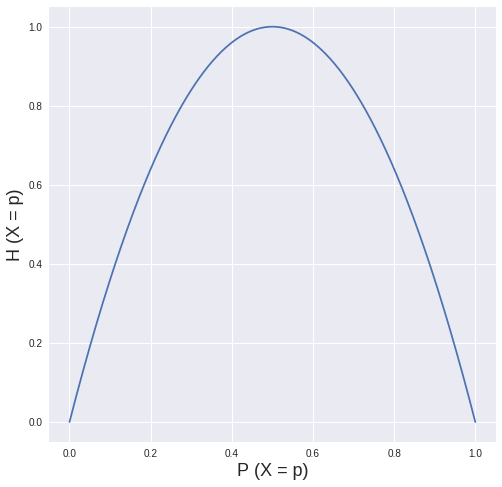
\includegraphics[scale=0.4]{figuras/entropy.png}
    \caption{Entropy}
    \label{fig:my_label}
\end{figure}

\end{frame}

\subsection{Kullback-Leibler Divergence}
\begin{frame}{{Theoretical Foundations - Kullback-Leibler Divergence}}

% \begin{align*}
%   \centering \textbf{Kullback-Leibler Divergence}
% \end{align*}

\begin{definition}


\begin{itemize}
    \item Given  a variable I, with probability distribution \textit{p}. It measures the error or divergence when it is assumed that the probability distribution of I is \textit{q}, instead of \textit{p}.
\end{itemize}


\begin{equation}
\label{eq:kullback}   
    KL_{I} = \sum_{i}^{n}p(i)log \frac{p(i)}{q(i)}
\end{equation}
\end{definition}
\end{frame}

\begin{frame}{Theoretical Foundations - Kullback-Leibler Divergence}
\begin{equation}
\label{eq:kullback_joint}   
    K_{I, J} = \sum_{i,j}^{n}p(i,j)log \frac{p(i,j)}{q(i,j)}
\end{equation}


\begin{equation}
\label{eq:kullback_cond}   
    K_{I \mid J} = \sum_{i,j}^{n}p(i,j)log \frac{p(i\mid j)}{q(i \mid j)}
\end{equation}


\end{frame}
\subsection{Mutual Information}
\begin{frame}{Theoretical Foundations - Mutual Information }
    \begin{definition}
    It is a measure derived from the Kullback-Leibler divergence. It is calculated between two processes \textit{I} and \textit{J} and quantifies the amount of information obtained about one process when observing the other. 

    
    It can be seen as the ``information produced by erroneously assuming that the two processes are independent''.\footnote{\cite{schreiber2000measuring}}

    \begin{equation}
        \label{eq:mutual}   
            MI_{I, J} = \sum_{i,j}^{n}p(i,j)log \frac{p(i,j)}{p(i)\cdot p(j)}
        \end{equation}
    \end{definition}

\end{frame}

\subsection{Transfer Entropy}
\begin{frame}{Theoretical Foundations - Transfer Entropy}
     \begin{definition}   
     It is a theoretical measure ``that shares some of the desired properties of mutual information but takes the dynamics of information transport into account''.\footnote{\cite{schreiber2000measuring}}
            
        \begin{equation} 
        \label{eq:trans-entropy}
        TE_{{J}->{I}} = \sum_{i,i_{t+h},j} p({i}_{t+h}, {i}_{t}^{k}, {j}_{t}^{l}) log\frac{p({i}_{t+h}\mid {i}_{t}^{k}, {j}_{t}^{l})}{p({i}_{t+h}\mid {i}_{t}^{k})}
        \end{equation} 
   \end{definition}

    
\end{frame}

\begin{frame}{Theoretical Foundations - Transfer Entropy}
        
        \begin{equation}
        \label{eq_ik}
            {i}^{k} =[{i_{t},...,{i}_{t-k+1}}] 
        \end{equation}
        
        \begin{equation}
        \label{eq_jk}
            {j}^{l}=[{j_{t},...,{j}_{t-l+1}}]
        \end{equation}

        \begin{itemize}
            \item It infers the veracity of the equation: 
        \end{itemize}

        

        \begin{equation}
            \label{eq:kullb}
                p({i}_{t+h}\mid {i}_{t}^{k}, {j}_{t}^{l}) =  p({i}_{t+h}\mid {i}_{t}^{k})
        \end{equation}
    
\end{frame}

\begin{frame}{Theoretical Foundations - Transfer Entropy}
Understanding of the parameters (Example)
    \begin{itemize}
        \item Series size = 6 samples
        \item k = 3 samples
        \item l = 2 samples
        \item h = 1 sample
        
    \end{itemize}
    
    \begin{figure}[!h]
        \centering
        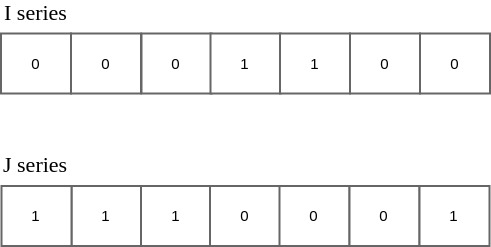
\includegraphics[scale=0.3]{figuras/series.png}
        \caption{I and J series.}
        \label{fig:series}
    \end{figure}
\end{frame}

\begin{frame}{Theoretical Foundations - Transfer Entropy}

    \begin{figure}[!h]
        \centering
        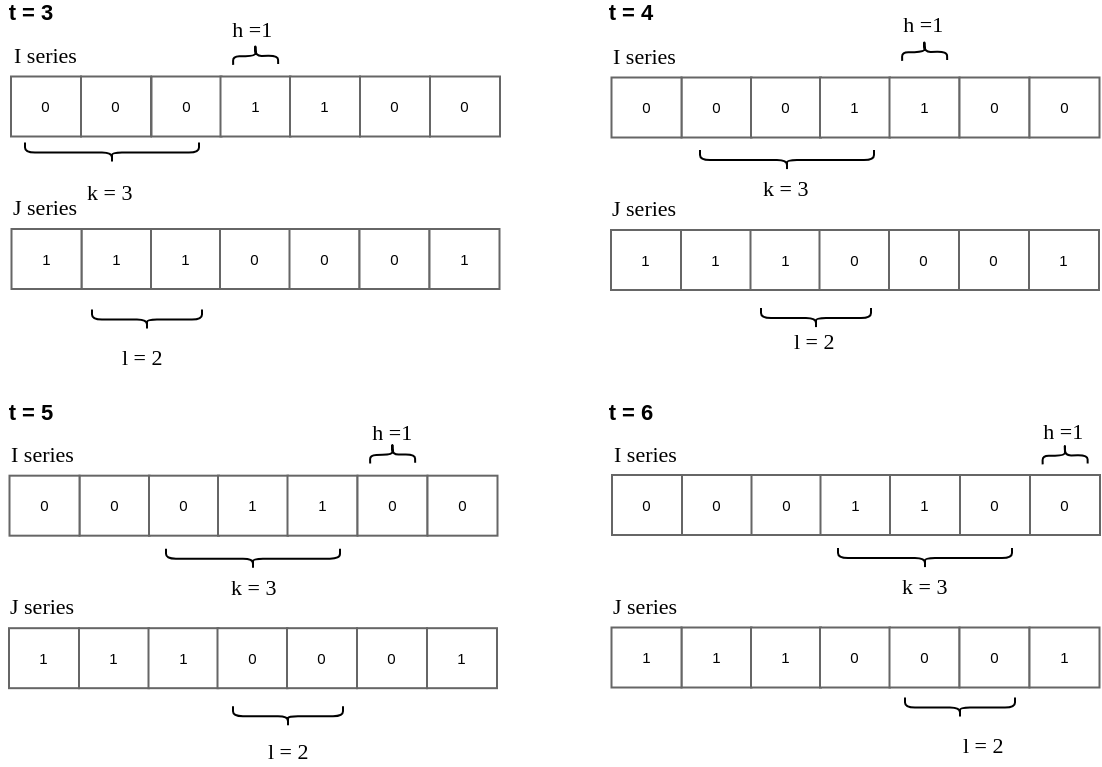
\includegraphics[scale=0.25]{figuras/te_sim.png}
        \caption{Choosing of the samples in TE.}
        \label{fig:te_sim}
    \end{figure}
\end{frame}

\subsection{Bayesian Networks}
\begin{frame}{Theoretical Foundations - Bayesian Networks}

    \begin{itemize}
        \item Probabilistic models based on direct acyclic graphs.
        \item The nodes represent variables of interest, while the connections represent relationships of informational or causal dependencies.\footnote{\cite{pearl2011bayesian}}
        \item Each variable is independent from its nondescendants, given its parents.
    \end{itemize}
\end{frame}

\begin{frame}
    \begin{itemize}
        \item {It factors the joint the distribution of the variable into local joint distributions.
        
        \begin{equation}
            P(A_n,\cap ... \cap A_1) = \prod_i^n P(A_i \mid \cap_{j=1}^{i-1}A_j)           
            \label{eq:bayes}
        \end{equation}

        \begin{equation}
            P(A_n,\cap ...\cap A_1) = \prod_{i=1}^n P(A_i|pa_i)
            \label{eq:compact_joint}
        \end{equation}

        \begin{equation}
             P(TbOrCa\mid Cancer,\ Bronch.,\ Asia) = P(TbOrCa \mid Cancer)
            \label{eq:ind_cond}
        \end{equation} 
        }
    \end{itemize}
\end{frame}

\begin{frame}{Theoretical Foundations - Bayesian Networks}
    \begin{figure}[!h]
        \centering
        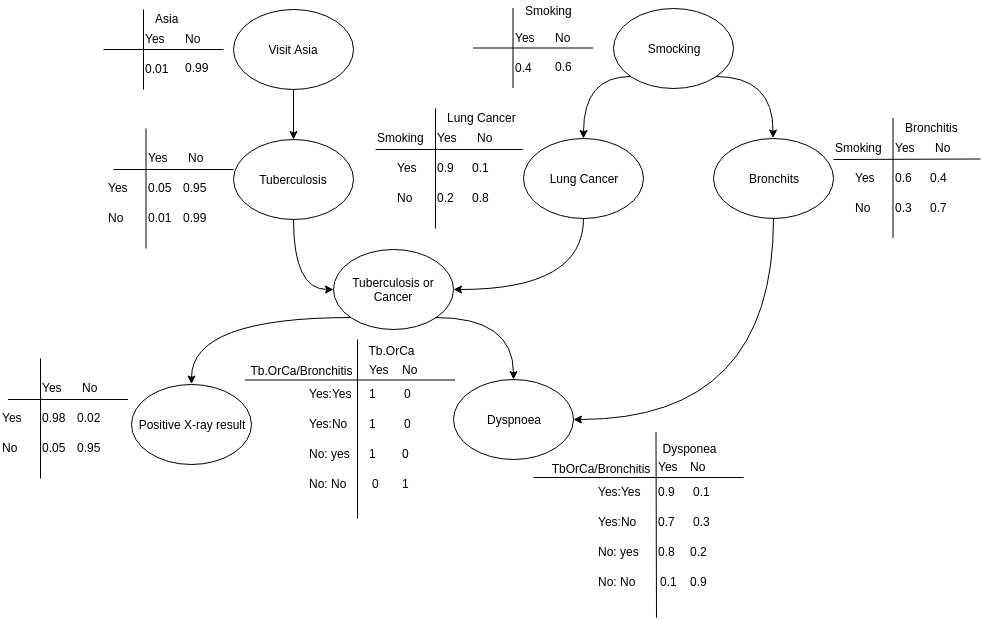
\includegraphics[scale=0.3]{figuras/asia_cpt.png}
        \caption{Bayesian Network Asia}
        \label{fig:asia}
    \end{figure}

\end{frame}



\subsection{Structural Learning}
\begin{frame}{Theoretical Foundations - Structural Learning}
 
\end{frame}

\subsection{K2-Algorithm}
\begin{frame}{Theoretical Foundations - K2 Algorithm}
    \begin{align*}
        \centering \textbf{ K2 - Algorithm}
    \end{align*}
    
    \begin{itemize}
        \item {Bayesian method for estimating a probabilistic network from data.}

        \item {The algorithm searchs for the network that has the highest posterior probability given a database of records.}
        \item {Necessity of a prior ordering on nodes.}
        \item { Scores each local network in order to find the most probable structure.}
        % \begin{equation}
        %     P(B_s, D) = c \prod_{i=1}^{n}\prod_{j=1}^{q_{i}}\frac{(r_i - 1)!}{(N_{ij} + r_i -1)!}\prod_{k=1}^{r_i}N_{ijk}!
        %  \label{eq:cooper-metric-gen}
        % \end{equation}
        % }
    \end{itemize}
    
\end{frame}

\begin{frame}


        \begin{columns}
	    \column{0.7\textwidth}\centering
        \begin{figure}[!h]
            \centering
            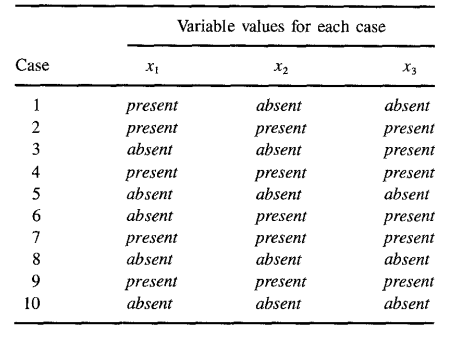
\includegraphics[scale=0.45]{figuras/cases_cooper.png}
            \caption{Database of cases}
            \label{fig:casesCoop}
        \end{figure}
        \column{0.3\textwidth}\centering
        \begin{figure}[!h]
            \centering
            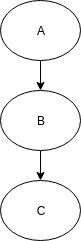
\includegraphics[scale=0.45]{figuras/typicOrder.png}
            \caption{Possible structure.}
            \label{fig:cases_graph}
        \end{figure}
	      
    \end{columns}
\end{frame}
    
\begin{frame}

\begin{figure}[!h]
            \centering
            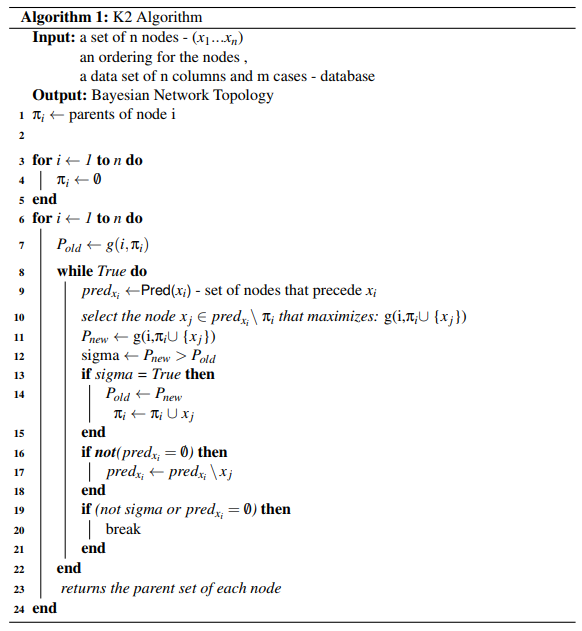
\includegraphics[height=72mm]{figuras/K2.png}
            \caption{K2-Algorithm}
            \label{fig:k2}
        \end{figure}
  
\end{frame}





